\chapter{Simulări și software folosit}
\label{chap:simulari}

\section{Dificultatea simulării unei rețele de apă}

Găsirea unui set de ecuații al cărei soluție să conducă la o estimare îndeajuns de bună pentru control este o condiție sine qua non pentru detecția unui defect și izolarea acestuia în cadrul nodurilor rețelei. Astfel după cum a fost expus în capitolul \ref{chap:intro} ecuațiile care guvernează relațiile intre viteza prin conducte și presiune dintr-un anumit punct sunt particularizări ale ecuațiilor Bernoulli-Euler sau Navier-Stokes. În cadrul unei rețele de apă a unui oraș, complexitatea rezolvării problemei crește semnificativ din varii motive precum:
\begin{itemize}
\item ansamblul de coduncte și noduri interconectate dă naștere unui sistem fizic greu de modelat matematic
\item parametrii care pot influența calitatea soluțiilor precum: tipul materialului conductei și al nodului, elevația fiecărui nod, rugozitatea fiecărei conducte și depunerile de pe aceasta
\item apariția unor factori exogeni care pot fi uneori greu de estimat - tiparul de utilizare al rețelei de către consumatori poate varia puternic
\item apariția defectelor precum scurgerile în proximitatea unui nod
\end{itemize}

Ținând cont de complexitatea problemei în regim dinamic pentru a putea obține o soluție de regim staționar a rețelei este necesar să ignorăm evenimentele imprevizibile precum apariția unei scurgeri sau variațiile bruște ale consumului.

Ecuațiile de regim staționar includ condiții de conservare fluxului de apă:

\begin{equation}
\label{Ecuația de conservare a rețelei de apă}
\sum\limits_{j=1}^{n} \mathbf B_{ij}\mathbf q_j=\mathbf d_i
\end{equation}

Unde $q_i$ reprezintă debitul prin fiecare conductă iar \textbf{B} reprezintă matricea de adiacență a rețelei la echilibru, definită astfel:
\begin{equation}
\textbf{B}_{ij} = 
     \begin{cases}
       1, & \text{conducta j intră în nodul i}\\
       0, & \text{conducta j nu este conectată la nodul i} \\
       -1, & \text{conducta j iese din nodul i}\\ 
     \end{cases}
\end{equation}

Partea de estimare a diferenței de presiuni (în engl. "Head-Flow differential") între două noduri interconectate se face utilizând formula Hazen-Williams ;\cite{sanz2016demand}:
\begin{equation}
\label{debit_presiune}
\mathbf h_i-\mathbf h_j=\frac{10.67\cdot L_\ell}{C_\ell^{1.852}\cdot D_\ell^{4.87}}\cdot \mathbf q_\ell\cdot |\mathbf q_\ell|^{0.852}
\end{equation}

unde:
\begin{itemize}
\label{Hazen-Williams}
\item $\textbf{h}$ reprezintă presiunea - măsurată de obicei în metru coloană de apă
\item $C_l$  reprezintă coeficientul de rugozitate al conductei
\item $D_l$ reprezintă diametrul conductei
\item $L_l$ reprezintă lungimea conductei
\item $q_l$ reprezintă debitul
\end{itemize}

Din ecuația empirică \eqref{Hazen-Williams} termenul $R_{ij}=\frac{10.67\cdot L_\ell}{C_\ell^{1.852}\cdot D_\ell^{4.87}}$ reprezintă rezistența conductei $ij$ iar dual, putem obține conductivitatea conductei $G_{ij} = \frac{1}{R_{ij}}$.

Având la dispoziție \eqref{Hazen-Williams} și \eqref{debit_presiune} putem exprima dependența debit presiune în regim staționar sub o formă matriceală compactă și cu o structură neliniară:

\begin{equation}
\label{eq:HW-matrix}
\mathbf B\mathbf G\left[\left(-\mathbf B^\top \mathbf h+\mathbf B_f^\top \mathbf h_f\right)\times \left|-\mathbf B^\top \mathbf h+\mathbf B_f^\top \mathbf h_f\right|^{-0.46}\right]=\mathbf d
\end{equation}


unde s-au luat în calcul și nodurile care au variații de presiune foarte mici - spre exemplu nodurile de tip tanc și  nodurile de tip rezervor - termenul $\mathbf B_f^\top \mathbf h_f$ reprezintă contribuția acestor noduri la starea de echilibru a rețelei.

Parametrul $\mathbf{d}$ reprezintă cosumul pentru noduri ($L/s$) și reprezintă un factor de incertitudine pentru întregul model. În cadrul unei simulări acesta poate fi estimat sau ales empiric, dar nu poate fi cunoscut cu precizie în fiecare moment. Problema aflării vectorului de consum a nodurilor intră în categoria problemelor legate de serii de timp și a estimării valorilor viitoare. Simulatoarele software transpun în general o variație a parametrilor de rețea (emitter-demand) în modificarea acestui parametru d.
% d este în general necunoscut, și se alege empiric, fiecare variație a demand-ului și a emitter-ului
% ceea ce se influențează de fapt în simulări este parametrul d, prin diferite variatii de emitter-demand

Din cauza dificultății rezolvării unei ecuații matriceale neliniare, software-ul specializat trebuie să folosească diferite metode de optimizare ("Solver") pentru a putea obține o diferență cât mai mică între cazul estimat și rezultatul real al ecuației. Este important de reținut faptul că rezolvarea problemelor de programare neliniară cu constrângeri poate generea de fapt o problemă NP-completă, sau în unele cazuri chiar NP-dură ;\cite{karp1975computational}.

\section{Simulări folosind biblioteca EPANET}

Dezvoltat la începutul anilor 90' de către USEPA (United States Environmental Protection Agency), EPANET a fost inițial privit ca un instrument pentru cercetare, acesta a devenit un standard de industrie la capitolul simulărilor software robuste pentru rețele de apă, foarte multe pachete software proprietare de simulare hidraulică se bazează masiv pe EPANET, diferențele apărând la design-ul interfeței grafice și a manipulării datelor. Aceast program de simulare oferă utilizatorului posibilitatea de a-și defini într-un mod interactiv o rețea de apă configurând tipul de nod, legătura între oricare două noduri și posibilitatea de a adăuga și elemente active în rețea, pompe. Pentru a simula utilizatorul trebuie să își definească pentru fiecare nod un anumit debit cerut de utilizatori, o elevație, și o legătură cu alte noduri. Simularea se va desfășura pe o perioadă de timp definită cu pasul de eșantionare cât mai convenabil ;\cite{rossman2000epanet}.
	
\begin{figure}[H]
\centering
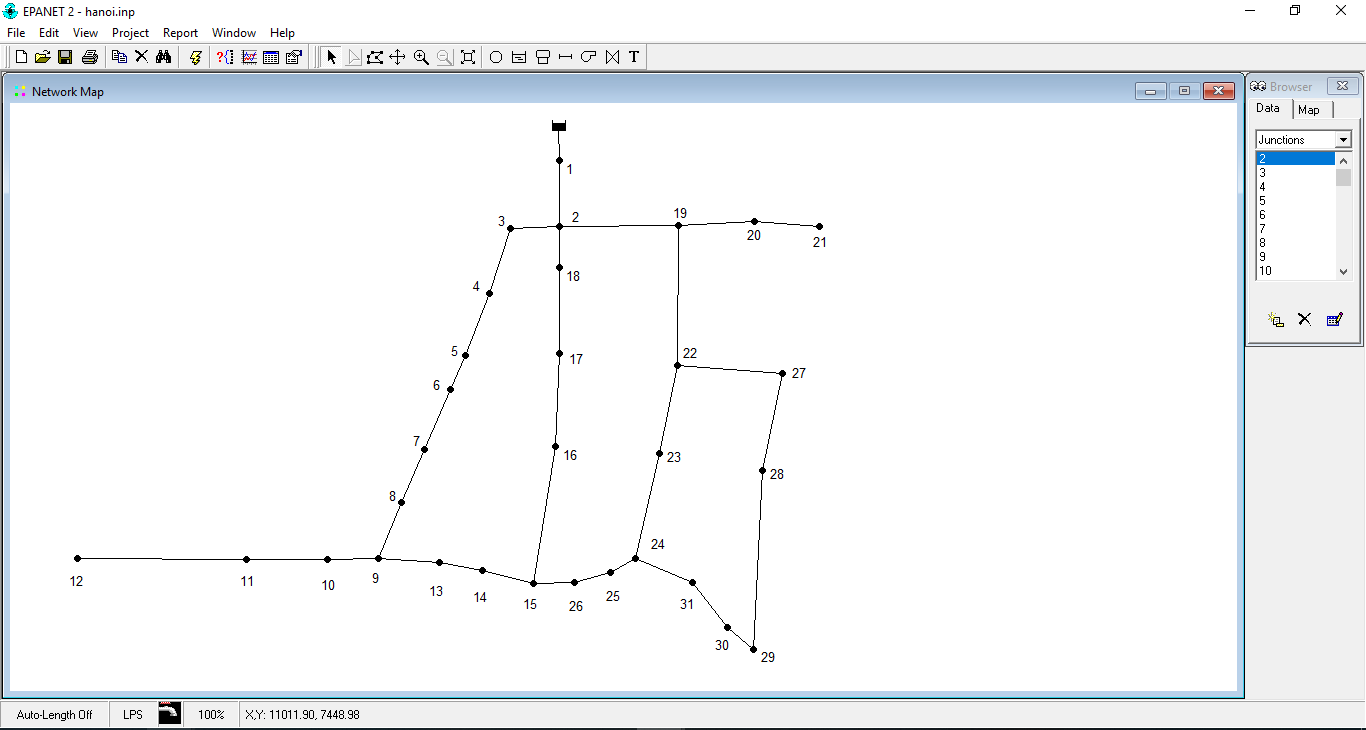
\includegraphics[width=0.75\textwidth]{pics/c2_pics/epanet_simulator.png}
\caption{Simulatorul EPANET}
\label{fig:epanet_simulator_win}
\end{figure}

În urma execuției simulării EPANET va stoca toate datele în memorie și va putea reliza grafice și alte interogări complexe.

Modalitatea în care simulatorul EPANET reușește să obțină datele de simulare este prin implementarea eficientă a ecuațiilor  Hazen-Williams \eqref{Hazen-Williams} Darcy-Weisbach și Chezy-Manning, la fiecare perioadă de eșantionare algoritmul bazat de metoda gradientului rezolvă ecuațiile matriceale neliniare.

Pe lângă posibilitatea de a simula în cadrul unui program de sine stătător toate scenariile dorite, USEPA pune la dispoziție și un API (Application Programming Interface) pentru a putea realiza programatic simulările și modificările aferente fiecărui scenariu. Folosind în acest fel interfața pusă la dispoziție scrisă în limbajul C și oferită sub forma unei biblioteci dinamice (în Windows fișier .dll, în Linux fișier .so) programatorul are posibilitatea de a realiza propriul software specializat pentru simularea rețelelor de apă. 

Particularizările programatice includ Demand-ul ( debitul de ieșire din nod către utilizatori L/s) fiecărui nod la orice moment de timp, proporționalitatea Demand-ului pentru a putea emula modul în care rețeaua este folosită de utilizatori de-a unei zile de lucru și unul din aspectele importante pe care EPANET le pune la dispoziție programatorilor este posiblitatea de a simula o scurgere în rețea emulată prin intermediul unui Emitter. Emitterul din biblioteca epanet este modelat ca un orificiu (perforație) prin care se poate scurge apa, fie din motive de a elibera presiunea sau din cauza unui defect. Ecuația care guvernează scurgerea prin acest orificu este:

\begin{equation}
\label{eq:emitter}
    q = Cp^\gamma
\end{equation}

unde:
\begin{itemize}
    \item q reprezintă debitul prin emitter
    \item C reprezintă o constantă de proporționalitate
    \item p reprezintă presiunea din joncțiune
    \item $\gamma$ reprzintă exponentul de presiune
\end{itemize}

Astfel apariția unui defect într-un anumit nod determină apriția unei relații liniare în funcție de presiunea din nod. Coeficientul $\gamma$ definde de tipul de joncțiune și de dimensiunea orificiului prin care se va scurge apa, pentru orificii relativ mici acesta ia valori de aproximativ 0.5 ;\cite{rossman2000epanet}.

\subsection{Schema bibliotecii ANSI C - EPANET}

API-ul pus la dispoziție se bazează pe funcții C scrise  într-o manieră modularizată, în ideea de a separa partea de analiză a rețelei și de modificare a parametrilor de partea de simulare hidraulică și calitativă. Astfel în imaginea de mai jos este prezentată modalitatea în care datele ajung și sunt folosite în cadrul simulatorului:

\begin{figure}[H]
\centering
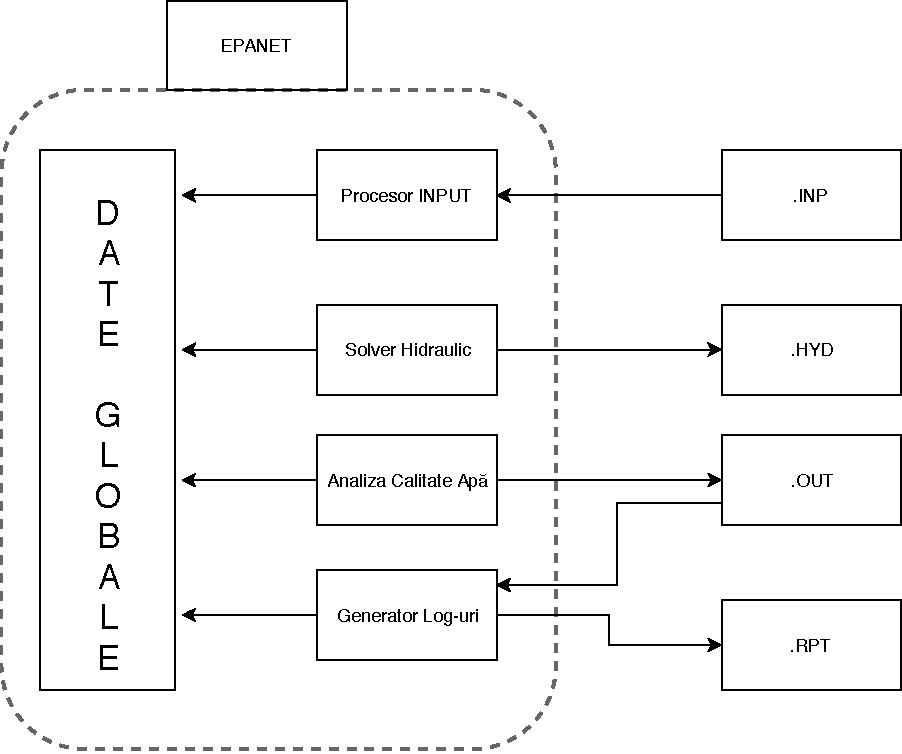
\includegraphics[width=0.75\textwidth]{pics/c2_pics/epanet_dataflow.pdf}
\caption{Fluxul de date în biblioteca EPANET}
\label{fig:EPANET_dataflow}
\end{figure}

\begin{flushleft}
Fișierele prezentate în schema de mai sus în partea dreaptă au semnificația:
\end{flushleft}
\begin{itemize}
    \item .INP - fișierul în care sunt definite topologia rețelei, tiparele de utilizare, caracteristicile elementelor active, valorile de Emitter și reguli complexe pentru funcționarea conductelor și pompelor
    \item .HYD - fișerul în care sunt stocate rezultatele simulării hidraulice
    \item .OUT - fișierul în care sunt stocate datele analizei calitative a apei
    \item .RPT - jurnalul în care biblioteca trece toate mesajele de eroare și atenționările cu privire la rețea
\end{itemize}

\subsection{Structura fișierului de intrare .INP}
Ceea ce stă la baza unei simulări este definirea input-ului rețelei de apă, anume fișierul INP. Fișierul INP - este un fișier text care conține anumite directive referitoare la componentele rețelei, 
tabelul de mai jos descrie toate aceste cuvintele cheie recunoscute de interpretor, împărțite în 4 categorii funcționale:

\begin{itemize}
    \item Componente - se definesc toate componentele fizice ale sistemului noduri, conducte, valve, emitters
    \item Simulare - se definesc caracteristicile care trebuie urmate de solver în procesul de simulare
    \item Calitate - se definesc parametrii relevanți analizei de apă - Cantitatea de substanță dizolvabilă din fiecare nod, constantele de timp pentru reacțiile de ordin I și II
    \item Jurnalizare - secțiune responsabilă cu fixarea parametrilor de execuție a rețelei - pasul de eșantionare, unitățile de măsură, parametrii impliciți și modul de raportare a simulării
\end{itemize}



\begin{table}[H]
\begin{tabular}{ p{3cm} p{3cm} p{3cm} p{3cm} }

Componente  & Simulare  & Calitate  & Jurnalizare \\
 \hline
 [TITLE] & [CURVES] & [QUALITY] & [OPTIONS] \\\
 \textcolor{blue}{[JUNCTIONS]} & \textcolor{blue}{[PATTERNS]} & [REACTIONS] & [TIMES] \\\
 [RESERVOIRS]& [ENERGY]& [SOURCES] &[REPORT] \\\
 [TANKS]& [STATUS] &[MIXING]& \\\
 \textcolor{blue}{[PIPES]} & [CONTROLS] &  &  \\\
 [PUMPS] & [RULES] &  & \\\
 [VALVES] & \textcolor{blue}{[DEMANDS]} & & \\\
 \textcolor{blue}{[EMITTERS]} & & &
\end{tabular}
\caption{Structura fișierului INP} \label{tabel:INP_Structure}
\end{table}


Cele mai importante directive au fost trecute în tabelul \ref{tabel:INP_Structure} în culoarea albastru. Urmând ca fiecare să fie explicată mai în detaliu.

\paragraph{[JUNCTIONS]} \mbox{} \\
Reprezintă structurile care definesc obiectele de tip nod din rețea, acestea vor avea ca atribute setate:
\begin{itemize}
    \item ID - indicele nodului
    \item Elevation - înălțimea nodului (m)
    \item Base demand - debitul inițial către utilizatori (s-a folosit termenul demand pentru a desemna cerința de apă din rețea)
    \item Demand pattern ID - pentru fiecare nod se poate fixa un anumit profil de utilizare prin legarea acestuia cu un anumit obiect PATTERN
\end{itemize}

\paragraph{[PIPES]} \mbox{} \\
Pipes reprezintă structurile care modelează conductele din rețea, pentru care atributele sunt:

\begin{itemize}
    \item ID - indexul fiecărei conducte
    \item Start node ID - indexul nodului de plecare
    \item End node ID - indexul nodului destinație
    \item Length - lungimea conductei (m)
    \item Diameter - diametrul conductei (mm)
    \item Roughness coef - coeficientul de rugozitate al conductei
    \item Minor loss coef - coeficientul de pierdere al conductei
    \item Status - conducta poate fi în 3 stări , deschisă - OPEN, închisă - CLOSED sau polarizată - CV (lasă să treacă fluxul de apă într-o singură direcție)
\end{itemize}

\paragraph{[EMITTERS]} \mbox{} \\
În lucrarea de față folosesc EMITTERS ca modalitate de a modela o scurgere de apă într-un anumit nod. Caracteristicile structurii sunt:
\begin{itemize}
    \item Junction ID - indexul nodului unde se află scurgerea
    \item Flow coeff - coeficientul C din ecuația \eqref{eq:emitter}
\end{itemize}


\paragraph{[PATTERNS]} \mbox{} \\
Prin intermediul structurilor PATTERN se definesc profilurile de utilizare ale rețelei. Modalitatea de funcționare a demand-ului este prin multiplicarea valorii PATTERN cu valoarea de Base Demand a fiecărui nod. Astfel motorul de simulare va diviza întreaga perioadă de simulare astfel încât fiecare multiplicitate să primească un interval de timp egal.

\paragraph{[DEMANDS]} \mbox{} \\
Structură care definește gradul de utilizare pentru fiecare nod din rețea. Atributele care definesc utilizarea sunt:
\begin{itemize}
    \item Junction ID - indexul nodului unde se dorește modificarea debitului de utilizare
    \item Base Demand - magnitudinea debitului de utilizare
\end{itemize}

\section{Integrarea EPANET cu Python}
Pentru a ușura mecanismul de procesare și interpretare am decis să folosesc funcțiile de bibliotecă EPANET adaptate din C la limbajul Python de proiectul open-source \cite{EpanetPython}. Motivele pentru care am ales limbajul Python sunt rapiditatea dezvoltării aplicației, robustețea soluției și ușurința tratării erorilor. Python este un limbaj interpretat - deci tipurile variabilelor sunt decise dinamic în momentul rulării aplicației în schimb acesta nu permite conversia implicită a variabilelor la run-time, eliminând astfel foarte multe erori greu de depistat.

Prin utilizarea unei clase de adaptare, \ref{lst:enwrap}, la API-ul de Python pus la dispoziție de \cite{EpanetPython} doresc să realizez o interfață mai ușoară pentru definirea, rularea simulărilor dar și pentru savlarea datelor într-un format care permite operabilitatea între mai multe programe, de exemplu Python-Matlab. Structura clasei de adaptare numită în engleză Wrapper (i.e. ambalaj al bibliotecii de funcții scrise în C) se bazează pe instanțierea unui obiect prin care se pot apela diferite funcții din biblioteca dinamică astfel încât să se obțină datele necesare.
Metoda clasei prin care se face interogarea rețelei este:

\lstinputlisting[language=Python,caption={Funcția de query},label={lst:queryfunc},firstline=105,lastline=105]{\code/ENWrapper.py}
Parametrul \textit{sim\_dict} primit de funcția \ref{lst:queryfunc} reprezintă un fișier JSON (Java Script Object Notation) care are o structură ce permite interogarea rețelei în legătură cu diferite mărimi dorite.

\lstinputlisting[caption={Structură JSON intrare},label={lst:inputJSON},firstline=109,lastline=119]{\code/ENWrapper.py}
Unde câmpurile reprezintă:
\begin{itemize}
    \item simulation\_name - numele simulării
    \item simulation\_type - tipul simulării H - hidraulic, Q - calitate a apei
    \item emitter\_values - un vector de cupluri (node\_index, emitter\_value), node\_index reprezintă indexul joncțiunii iar emitter\_value reprezintă magnitudinea scurgerii din acel nod
    \item query - reprezintă valorile care se doresc a fi interogate pentru fiecare componentă:
    \begin{itemize}
        \item EN\_PRESSURE - întoarcerea valorilor presiunilor pentru fiecare nod
        \item EN\_DEMAND - întoarcerea valorilor demand-ului pentru fiecare nod
        \item EN\_VELOCITY - întoarcerea valorilor vitezei apei prin fiecare conductă
    \end{itemize}
\end{itemize}
La apelarea funcției query\_network se va returna de asemenea un dicționar, care poate fi convertit la format-ul JSON, pentru a putea fi folosit în alte procese de simulare și validare, spre exemplu într-un mediu de dezvoltare Matlab/Octave. Structura fișierului de ieșire este:



\lstinputlisting[caption={Structură JSON ieșire},label={lst:outputJSON},firstline=122,lastline=132]{\code/ENWrapper.py}
Câmpul NODE\_VALUES reprezintă un vector JSON-uri, fiecare element al acestui vector fiind în fapt rezultatul numeric al unei simulări pentru câmpurile specificate la fișierul de intrare \ref{lst:inputJSON}.

Un pas important în dezvoltarea Wrapper-ului peste EPANET a reprezentat tratarea erorilor returnate de funcțiile de C. În momentul apelării unei funcții de C, EPANET returnează o pereche (a, b) unde a reprezintă valoarea efectivă interogată iar b reprezintă codul erorii. Tratarea excepțiilor s-a făcut cu ajutorul funcției:

\lstinputlisting[caption={Cod pentru tratarea erorilor},label={lst:errorcheck},firstline=298,lastline=312]{\code/ENWrapper.py}

și prin definirea unei excepții customizate pentru clasa ENWrapper scrisă

\lstinputlisting[caption={Definirea Excepției},label={lst:enexception},firstline=333,lastline=336]{\code/ENWrapper.py}

\section{Simulări pe rețeaua de apă din Hanoi}

Având ca susținere fișierul pentru rețeaua de apă din Hanoi \ref{fig:hanoinetwork} și biblioteca EPANET cu codul de
adaptare Python, pot realiza simulări asupra acestei rețele de apă. Inițial voi explicita profilurile de utilizare a
rețelei de apă urmând ca mai apoi să arăt modul în care rețeaua funcționează în mod nominal (fără nici un defect).

Parametrii funcționali rețelei hanoi.inp sunt următorii:

\begin{itemize}
    \item pasul de eșantionare al simulării 15min
    \item pasul de eșantionare al pattern-ului 15min
    \item Perioada de simulare este de 24h
\end{itemize}

Graficul de utilizare al rețelei are o distribuție centrată în jurul orelor dimineții - acest lucru fiind corelat cu faptul că atunci este momentul în care cei mai mulți utilizatori își încep activitatea și consumă apă. Astfel rețeaua este supusă unui stres mai mare în timpul orel matinale față de exemplu de perioada nopții unde valorile multiplicității ajung la valori aproximativ de două ori mai mici.

\begin{figure}[H]
  \centering
  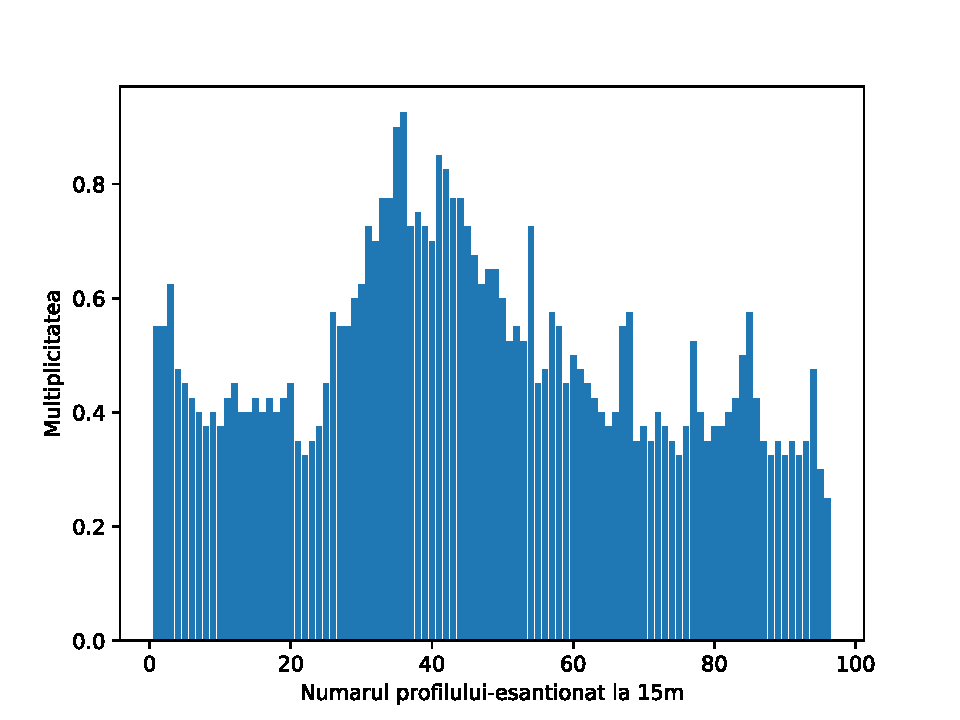
\includegraphics[width=0.75\textwidth]{\pics/c2_pics/profil_normal.pdf}
  \caption{Profilul normal de utilizare}
  \label{fig:normalprofile}
\end{figure}

Pentru rularea unei simulări nominale fișierul JSON de intrare poate avea câmpul de emitter\_values gol, obținându-se asftel caracteristica tranzitorie a presiunii, a debitului din noduri și a vitezei fluxului de apă din conducte.


\section{Prezentarea măsurilor de interes preluate din simulări}

Problema care se pune în continuare alegera unui subset din mărimile prelevate din simulator astfel încât discernerea între un caz de utilizare normal și unul defectuos să fie cât mai ușoară. 


\subsection{Simulare dinamică pentru încărcare nominală}
În regim nominal ansamblul rețelei de apă nu este supus la nici un defect, funcționarea fiind corespunzătoare profilului de utilizare normal \ref{fig:normalprofile}. Datele care sunt extrase din simularea nominală și prezintă interes pentru analiză sunt corespunzătoare presiunii din fiecare nod. De asemenea vor fi prezentate și celelalte măsurători - viteza apei prin conducte și debitul către utilizatori.

\begin{figure}[h]
\centering
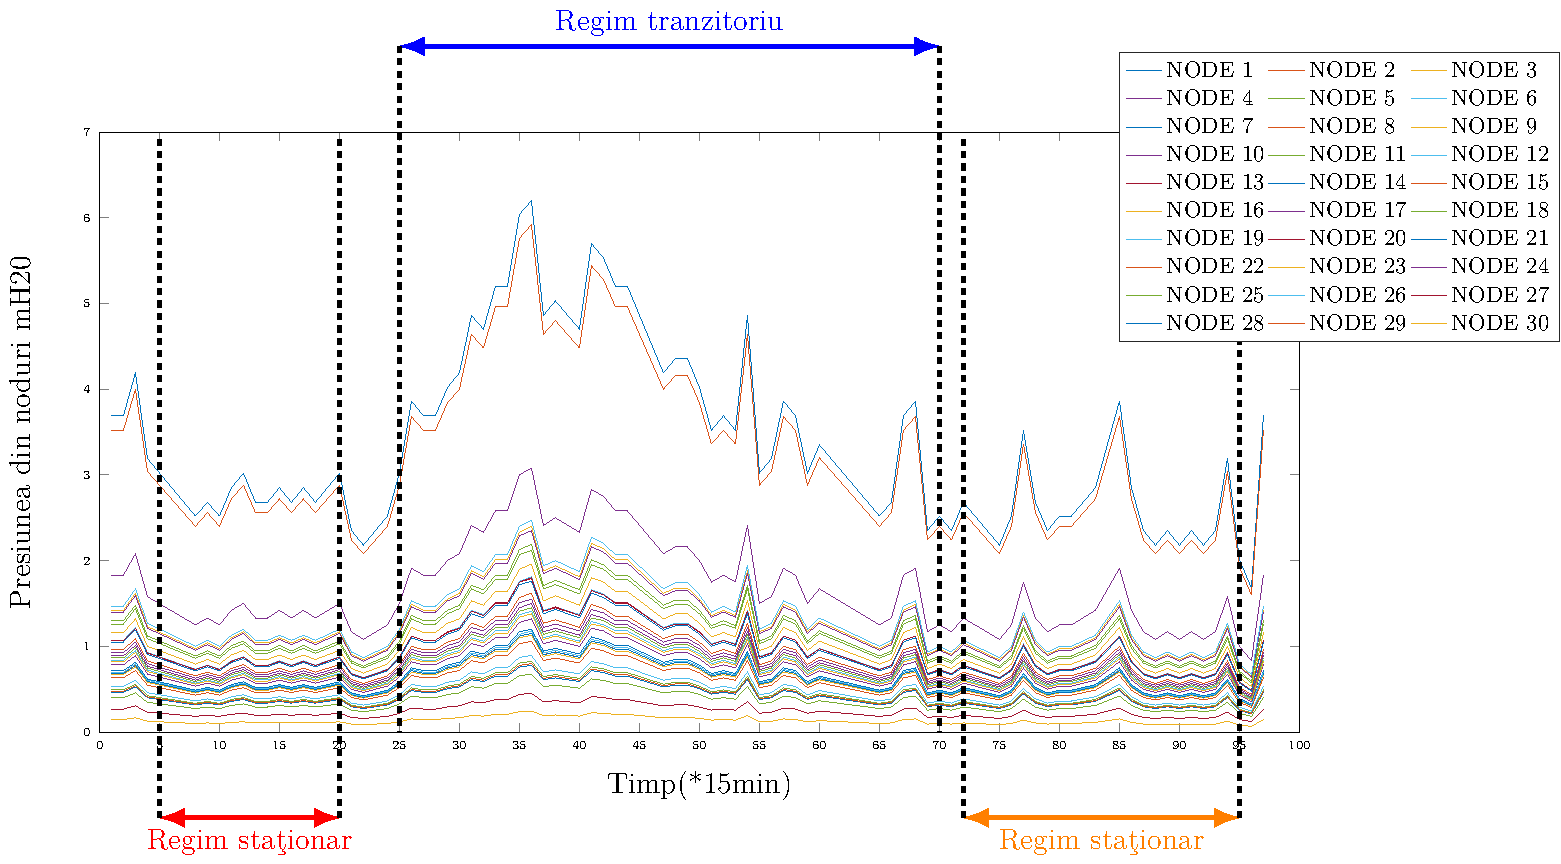
\includegraphics[width=0.90\textwidth]{\pics/c2_pics/ref_pressure/reference_pressure.pdf}
\caption{Profilul nominal al presiunii}
\label{fig:ref_presssure}
\end{figure}

După cum se poate observa în \ref{fig:ref_presssure} profilul nominal al presiunii intră în tiparul profilului de cerere prezentat în \ref{fig:normalprofile}, unde în jurul orelor dimineții, când activitatea utilizatorilor este asociată unui regim dinamic al rețelei, iar orele nopții sunt caracterizate de marimi lent variabile. Astfel pe acest grafic s-au putut evidenția 3 zone importante, anume, cele două zone de regim staționar în intervalele $[5, 20] *15min$ și $[72,95]*15min$ și zona de regim dinamic în intervalul $[23,70]*15min$. Este de menționat că aceste intervale au fost selectate empiric în baza unei analize grafice asupra caracteristicilor presiune-viteză-debit.

\subsection{Alte mărimi de interes din simulatorul EPANET}

Caracteristicile de viteză și debit urmează o caracteristică asemănătoare cu caracteristica de presiune din fiecare nod, o explicație naturală provenind de la faptul că presiunea este considerată ca fiind înălțimea nivelului de apă dintr-un nod.

\begin{figure}[H]
\centering

\subfloat[Profil nominal demand]{%
  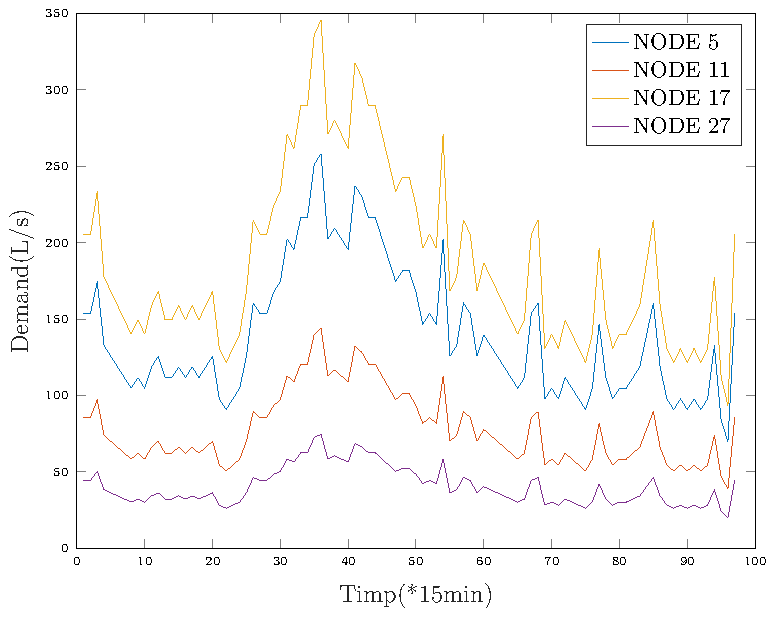
\includegraphics[width=0.45\textwidth]{\pics/c2_pics/ref_others/ref_demand}%
  \label{fig:ref_demand}%
}\qquad
\subfloat[Profil nominal viteza]{%
  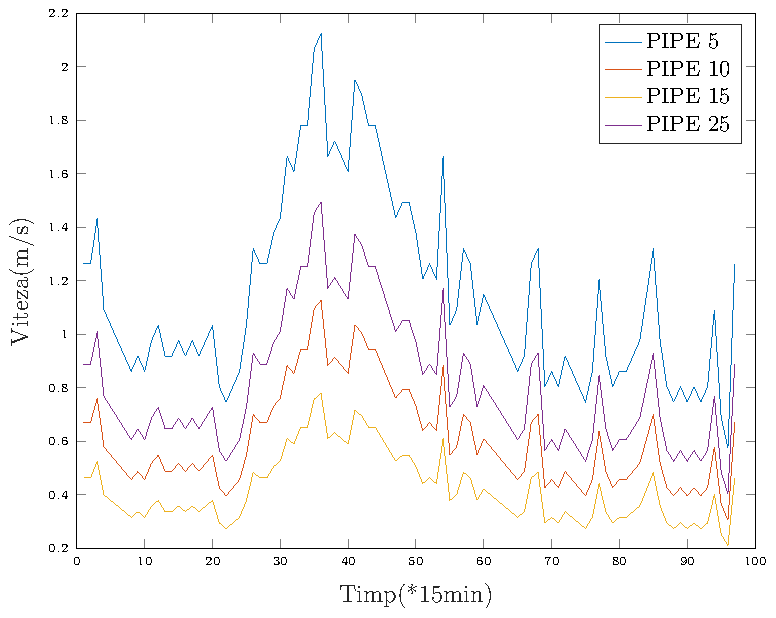
\includegraphics[width=0.45\textwidth]{\pics/c2_pics/ref_others/ref_velocity}%
  \label{fig:ref_pressure}%
}

\caption{Rezultate simulări nominale}
\label{fig:ref_demand_vel}
\end{figure}

După cum se observă în \ref{fig:ref_demand_vel} zonele de regim staționar și de regim dinamic se păstrează în continuare și pentru caracteristicile de viteză și debit. De asemenea este important de menționat că profilurile nominale ale celoralte noduri decât cele ilustrate în figurile de mai sus urmează aceeași caracteristică dinamică, alegerea nodurilor și conductelor respective a fost făcută pentru a păstra figura curată.




